\chapter{Problem 1}
  \section{Problem 1a}
	
	From the z-transform of the described filter in Problem 1 we get:
	\begin{equation}
		X(z)=\rho X(z)z^{-1}+\sqrt{1-\rho ^2}*E(z) 
		\label{eq:eq_impulse_response}
	\end{equation}
	If we sort equation~\ref{eq:eq_impulse_response} in regard of $\frac{X(z)}{E(z)}$ we get:
	\begin{equation*}
		\frac{X(z)}{E(z)}=T(z)=\frac{\sqrt{1-\rho ^2}}{1-\rho z^{-1}}	
		\label{eq:eq_freq_resp_x}
	\end{equation*}
	
	Make the z-transform back to the diskrete plane
	
	\begin{equation*}
		t(n)=\sqrt{1-\rho ^2}\rho ^nu(n)
	\end{equation*}
	
	Since the noise is uncorrolated, we may reduce the convolution to find x(n)
	
	\begin{equation*}
		x(n)=t(n)\Asterisk e(n)=t(n)\sigma ^2_W
	\end{equation*}
	
	From Problem 1 it is given that
	
	\begin{equation*}
		\sigma ^2_W=1
	\end{equation*}
	
	This results in equation~\ref{eq:eq_AR_process}.
	
	\begin{equation}
		x(n)=\sqrt{1-\rho ^2}\rho ^nu(n)
		\label{eq:eq_AR_process}
	\end{equation}
	
	From the output calculated in equation~\ref{eq:eq_AR_process} we may use the following equation~\ref{eq:eq_autocorrelation_compendium} from the compendium to calculate the autocorrelation:
	
	\begin{equation}
		R_x(\tau)=\sum_{n=-\infty}^{\infty}E\{x(n)\}E\{x(n+\tau)\}
		\label{eq:eq_autocorrelation_compendium}
	\end{equation}
	
	By inserting our definition of x(n) we get equation~\ref{eq:autocorrelation_x}.
	
	\begin{equation}
		R_x(\tau)=(1-\rho ^2)\sum_{n=0}^{\infty}\rho ^n\rho^{n+\tau}
		\label{eq:autocorrelation_x}
	\end{equation}
	
	By using the formula for geometric series we get equation~\ref{eq:autocorrelation}
	
	\begin{equation}
		R_x(\tau)=(1-\rho ^2)\rho^{\tau }\sum_{n=0}^{\infty}\rho^{2n}=(1-\rho ^2)\rho^{\tau }\frac{1}{1-\rho ^2}
		\label{eq:autocorrelation}
	\end{equation}
	
	After shorting equation~\ref{eq:autocorrelation} we get equation~\ref{eq:autocorrelation_complete} that is shown in figure~\ref{fig:autocorrelation}.
	
	\begin{equation}
		R_x(\tau)=\rho^{|\tau |}
		\label{eq:autocorrelation_complete}
	\end{equation}

	
	\begin{figure}[H]
	  \centering
	  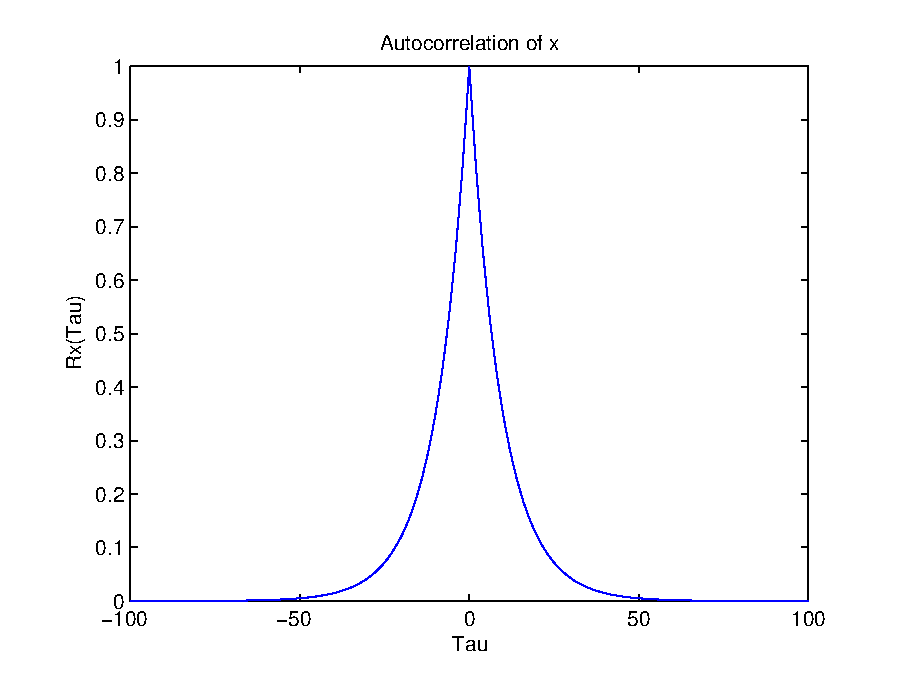
\includegraphics[width=0.75\textwidth]{img/Oppgave1a}
	  \label{fig:autocorrelation}
	\end{figure}
	
  
  
  \section{Problem 1b}
	The power spectral density may be given by equation~\ref{eq:spectral_density} where T(f) is the AR filter process:
	\begin{equation}[H]
		Sx(f)=|T(f)|^2=T(f)T^*(f)
		\label{eq:spectral_density}
	\end{equation}
	
	Insert the expression from equation~\ref{eq:eq_freq_resp_x} and calculate:
	
	\begin{equation*}[H]
		T(f)=T(z)|_{z=e^{j2\pi f}}=\frac{\sqrt{1-\rho ^2}}{1-\rho e^{-j2\pi f}}
	\end{equation*}
	
	Expanding the denominator and cleaning up.
	
	\begin{equation*}[H]
		Sx(f)=\frac{\sqrt{1-\rho ^2}^2}{(1-\rho e^{-j2\pi f})(1-\rho e^{j2\pi f})}=\frac{1-\rho ^2}{1-\rho e^{j2\pi f}-\rho e^{-j2\pi f}+\rho ^2}
	\end{equation*}
	
	Using eulers formula for cosine function to reduce to equation~\ref{eq:eq_Spectral_Density_X} and plot the result in figure~\ref{fig:power_spectral_density_x}.
	
	\begin{equation}[H]
		Sx(f)=\frac{1-\rho ^2}{1+\rho ^2-2\rho cos(2\pi f)}
		\label{eq:eq_Spectral_Density_X}
	\end{equation}
	
	\begin{figure}[H]
	  \centering
	  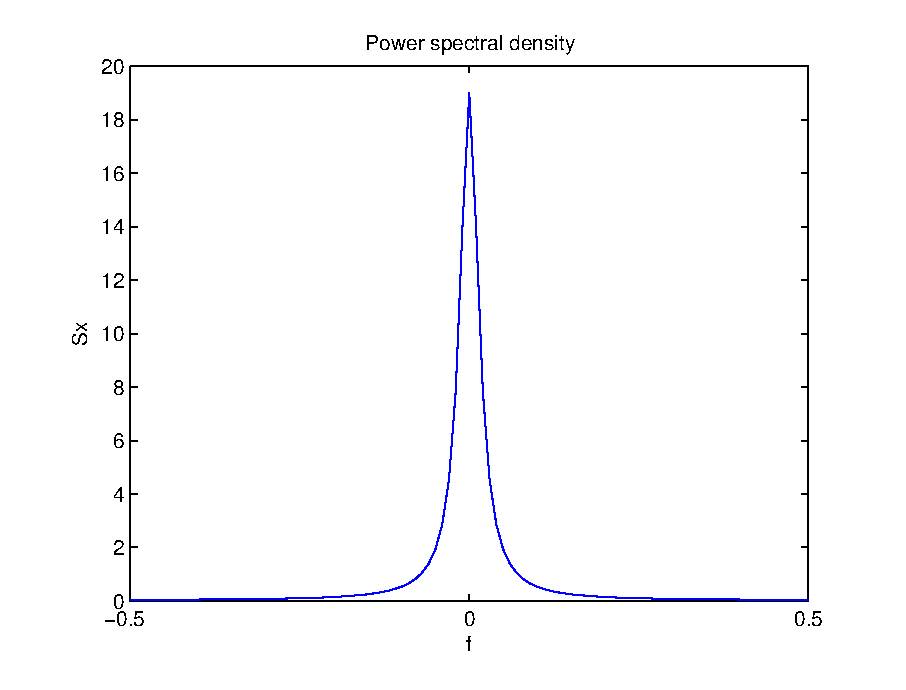
\includegraphics[width=0.75\textwidth]{img/Oppgave1b}
	  \label{fig:power_spectral_density_x}
	\end{figure}
  
  \section{Problem 1c}
	The matlab code for this function is placed in appendix~\ref{app:1c}.
	
  
  \section{Problem 1d}
	
	\begin{figure}[h]
	  \centering
	  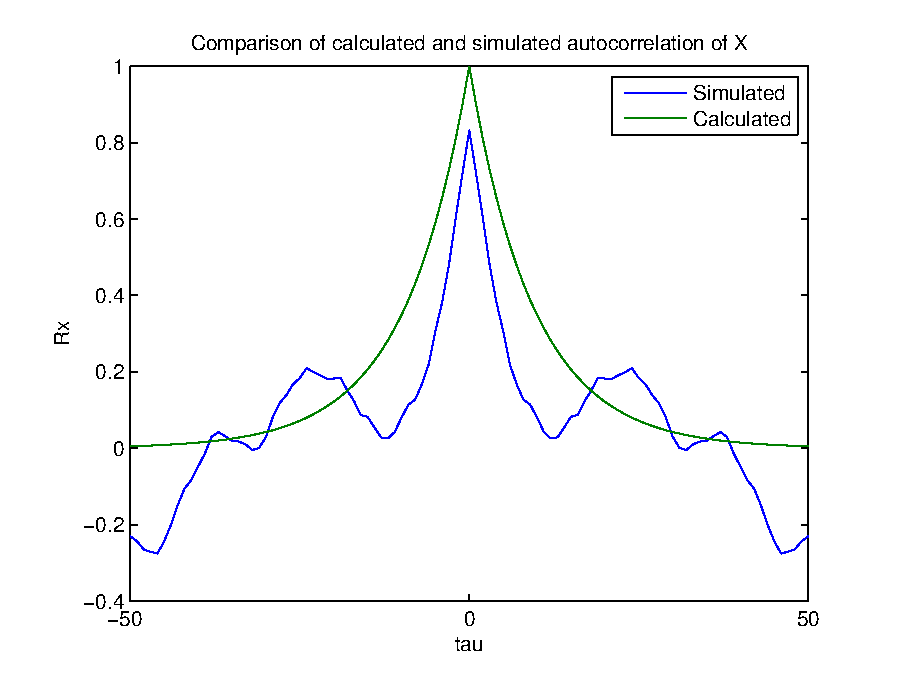
\includegraphics[width=0.75\textwidth]{img/Oppgave1d}
	  \label{fig:oppave1d}
	\end{figure}
	
	As seen in figure~\ref{fig:oppave1d}, the simulated and calculated autocorrelations are similar. Some variation may be seen between each run of the script. 
  
  \section{Problem 1e}
	
	\begin{figure}[h]
	  \centering
	  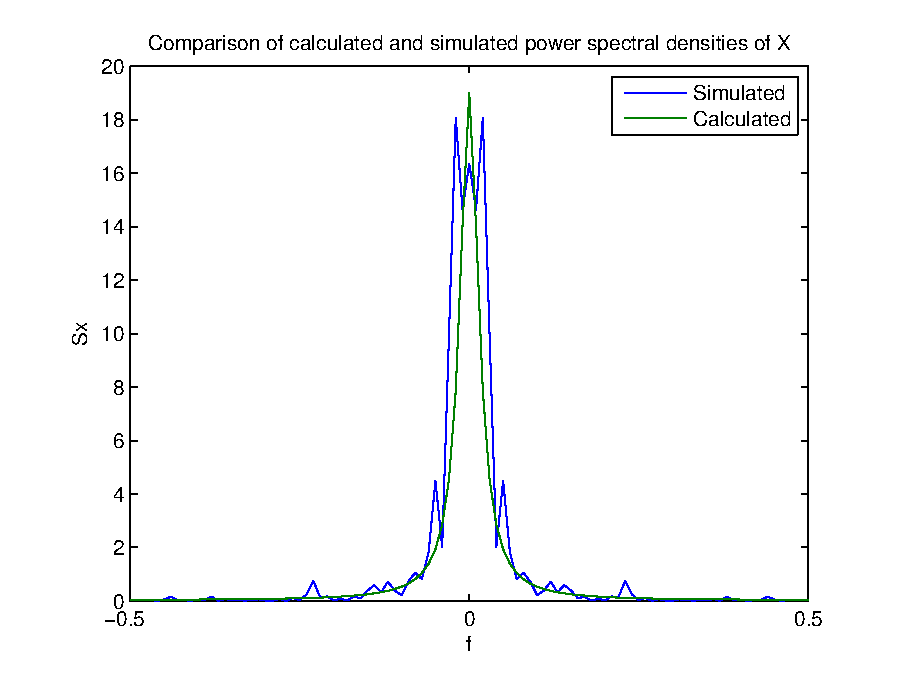
\includegraphics[width=0.75\textwidth]{img/Oppgave1e}
	\end{figure}
	
	When calculating the fft of the output, we had to use a limited amount of samples to achieve normal results. This was to limit the amount of noise in the plot.
	Again, there will be some variation between each run of the script, but after some runs it became apparent that the result were approved.